\chapter{Analisi del Rumore In Ingresso}\label{cap:rumore}

Il primo passo per analizzare il segnale audio in ingresso è quello di valutare il rumore presente durante la registrazione effettuata dalla scheda audio. 
A questo scopo sono state realizzate diverse registrazioni in assenza di segnale utile. 

In condizioni standard, cioè in assenza di disturbi a particolari frequenze, il rumore di registrazione può essere definito come rumore rosa.
La figura \ref{fig:rumore} mostra lo spettro del rumore presente durante una registrazione.
Dall'immagine si può notare come l'energia sia più concentrata nelle basse frequenze, in particolare nella componente continua, e diminuisca gradualmente man mano che la frequenza aumenta.

%Inoltre, dal momento che non si può escludere la presenza di disturbi esterni casuali concentrati in particolari frequenze, si è cercato di isolare il più possibile la zona di registrazione da tali disturbi, in modo tale da mantenere l'intensità di questi suoni inferiore rispetto a quella del segnale utile.
 
%Si discuterà del filtro utilizzato per ridurre il rumore nel capitolo \ref{cap:rilevamento_frequenza}.
	\begin{figure}[h]
	  \begin{center} 
	    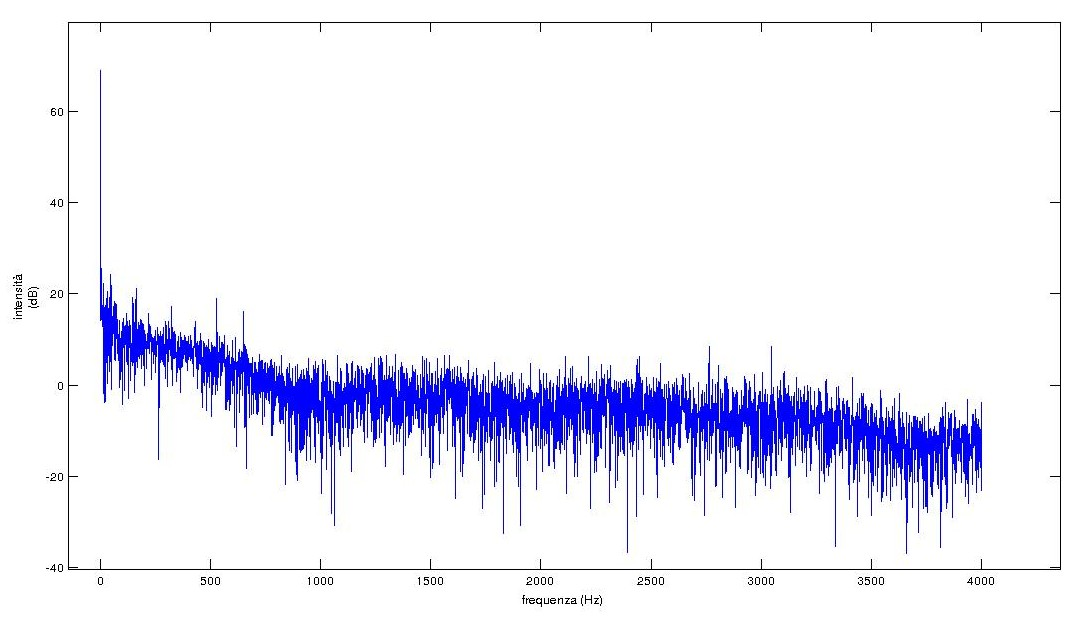
\includegraphics[width=\textwidth*\real{0.9}]{images/ch_02/spettro_rumore.jpg}
	  \end{center} 
	  \caption{\textit{Rumore di registrazione}}  
	  \label{fig:rumore}
	\end{figure}



